\section{Extensive game with imperfect information}

n many strategic settings, players are required to make decisions without full knowledge of the prior actions taken by others. 
This lack of information—such as when players move simultaneously. 
Despite this, such scenarios can still be modeled using a game tree.
\begin{figure}[H]
    \centering
    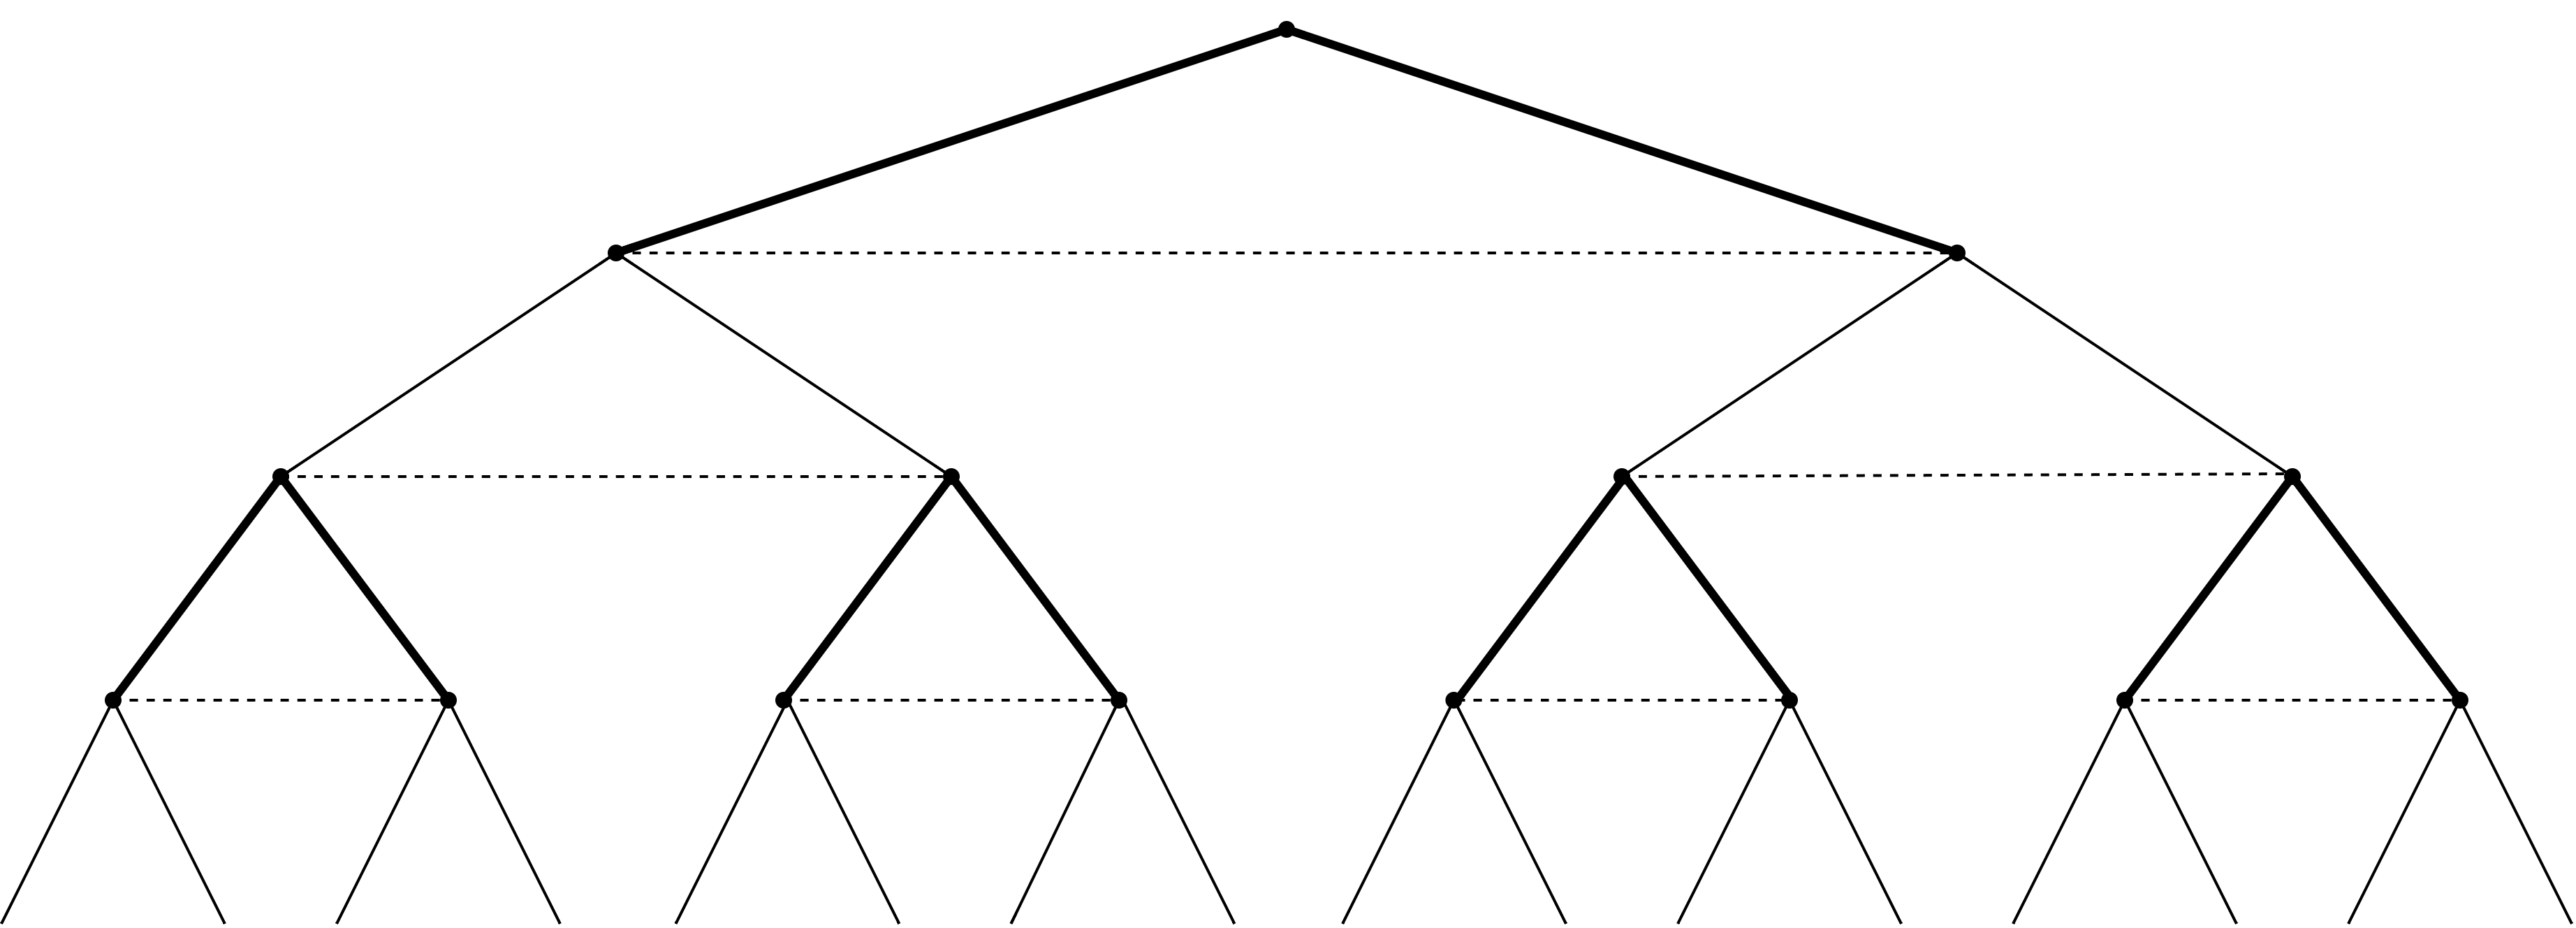
\includegraphics[width=0.75\linewidth]{images/gt.png}
    \caption{Extensive game with imperfect information}
\end{figure}
In the figure, dashed lines connect nodes that are indistinguishable to a player. 
That is, the player knows they are at one of the connected nodes, but cannot tell which one specifically.
\begin{definition}[\textit{Information set}]
    An information set for Player $i$ is a pair $(U_i, A(U_i))$ satisfying the following conditions: 
    \begin{enumerate}
        \item $U_i \subset P_i$ is a non-empty set of vertices $v_1, \cdots, v_k$.
        \item Each vertex $v_j\in U_i$ has the same number of children.
        \item $A_i(U_i)$ is a partition of the children of $v_1 \cup \dots \cup v_k$ such that each element of the partition contains exactly one child from each vertex $v_j$.
    \end{enumerate}
\end{definition}
\noindent Intuitively, an information set represents the player's uncertainty about their exact position in the game tree. 
The associated partition $A(U_i)$ defines the available actions.
\begin{definition}[\textit{Extensive game with imperfect information}]
    An extensive-form game with imperfect information consists of the following elements:
    \begin{enumerate}
        \item A finite set of players $N = \{1, \dots, n\}$.
        \item A game tree $(V, E, x_0)$. 
        \item A partition of the non-terminal (non-leaf) nodes into sets $P_1, P_2, \dots, P_{n+1}$.
        \item A partition $(U^j_i), j = 1, \dots, ki$ of the set $P_i$, for all $i$, with $(U^j_i, A^j_i)$ being the information set for all players $i$ at all vertices $j$ (having the same number of children). 
        \item A probability distribution defined for each vertex in $P_{n+1}$ on the edges leading to its children.
        \item An $n$-dimensional vector assigned to each leaf.
    \end{enumerate}
\end{definition}
\noindent Note that when all information sets contain singletons, the game reduces to one with perfect information.
\begin{definition}[\textit{Pure strategy}]
    A pure strategy for Player $i$ in an imperfect information game is a function defined over the collection $\mathcal{U}$ of their information sets, assigning to each $U_i\in\mathcal{U}$ an element from the partition $A(U_i)$. 
\end{definition}
\begin{definition}[\textit{Mixed strategy}]
    A mixed strategy is defined as a probability distribution over the pure strategies.
\end{definition}